\newcommand{\video}[2]{\href{#1}{Vídeo: #2}}

% Erros que serão repetidos/reutilizados em mais de um local
\newcommand{\erroArmazenarSenhaAberta}[0]{armazenamento de senhas abertas (ou com criptografia reversível) no banco de dados sem \textit{hash} \cite{password_storage_cheat_sheet}}    



\chapter{Erros comuns em projetos}
\label{erros-projetos}

Nesse capítulo estão apresentados os erros mais comuns que os professores observam nos sistemas desenvolvidos nas disciplinas de projetos. Alguns fazem parte de mais de uma categoria, mas foram listados cada um em uma categoria representada pela seção do documento.

São apresentados alguns problemas de projeto / modelagem e outros específicos do desenvolvimento.

Algumas referencias indicadas nesse capítulo são de publicações e vídeos disponíveis na internet que devem ser lidas / assistidos para correta compreensão do contexto.

O formato desse capítulo não segue exatamente o formato de documento indicado para os trabalhos acadêmicos.

\todo[inline]{Colocar aqui os erros mais comuns nos projetos de software das disciplinas}

\section{Erros relacionados a Arquitetura / Provedor de serviços}

Cada projeto deve buscar uma arquitetura compatível com seus objetivos, tanto em termos de capacidade como em termos de custos. A escolha do provedor de serviços deve ser feita com cuidado, considerando custos, conhecimentos da equipe e funcionalidades oferecidas. As maquinas devem ser dimensionadas corretamente de forma que não existam grandes custos.

Alguns ambientes oferecem serviços de forma gratuita sem cartão de crédito e outros solicitam forma de pagamento. Nos provedores de serviços com custos variáveis é importante fazer acompanhamento diário do uso e dos custos e escolher corretamente os serviços que são contratados. Utilizar os serviços no sistema aberto em vez das opções acadêmicas/gratuitas pode ser mais simples mas resultar em custos indesejados. 

As escolhas dos serviços devem considerar a real necessidade de uso de forma a ter um uso racional dos recursos. Mesmo um serviço disponibilizado de forma gratuita tem um custo para o provedor e consome energia para funcionar. O abuso no uso dos serviços oferecidos pode gerar limitações futuras e consumir recursos energéticos sem necessidade.

Muitos detalhes que devem ser pensados na definição de arquitetura são apresentados por \citeauthoronline{como_fazer_ingresso_com_escalar} no video \citetitle{como_fazer_ingresso_com_escalar}, esses detalhes vão garantir eficiência no uso de recursos e ainda atender corretamente o usuário da aplicação. Apesar desse vídeo apresentar uma situação que não é tão comum os conceitos se aplicam em praticamente em todos os projetos, saber as possibilidades permite que escolhas corretas sejam feitas.


\section{Erros de Processo}

Os processos da aplicação devem ser desenvolvidos de forma que o usuário possa utilizar a aplicação de maneira simples e intuitiva, existem casos onde o processo atual pode ser redefinido e criar ganhos, mas existem casos onde não é possível redefinir o processo real e o sistema deve atender a esse processo.

Muitas vezes o analista e o desenvolvedor não se colocam no papel do usuário para verificar se o que estão desenvolvendo faz sentido para quem vai realmente utilizar a aplicação. 

\begin{itemize}
    \item interface que não trata o processo de forma simples para o usuário (somente \gls{crud} e o usuário precisa saber qual sequencia deve utilizar);
    
    \item muitas bibliotecas e padrões abertos facilitam o desenvolvimento e simplificam a aplicação, normalmente não existe justificativa para \enquote{reinventar a roda}, ex: 
      \begin{itemize}
          \item utilização de \enquote{login social} OAuth;

          \item utilizações de bibliotecas para tratamentos básicos de segurança;
          
          \item utilizações de bibliotecas para validações;
          
          \item utilização de Gravatar para imagem de perfil.
      \end{itemize}
\end{itemize}

\section{Erros de Segurança}

\begin{itemize}
    \item não seguir recomendações de ferramentas de análise estática e \ac{owasp}, um importante ponto de partida é a leitura de \citetitle{owasp_cheat_sheet};

    \item implementação de um processo de recuperação de senha que depende de dados públicos : 
    Caso real que aconteceu com o sistema do \ac{enem} - \citetitle*{medicina_cachaca}  \cite{medicina_cachaca};

    \item implementação de um processo de autenticação que depende somente de dados públicos - Caso real em setembro/2021 onde um e-commerce utiliza somente CPF e e-mail para \enquote{autenticação} e com esses dados era possível ter acesso a endereço, telefone, bandeira e número final de cartão de crédito e dados dos pedidos. O atendimento do e-commerce informou que não era possível utilizar senha, que o concorrente utilizava o mesmo processo e que os clientes não queriam saber de senha. Ao entrar em contato com a empresa desenvolvedora essa disse que a responsabilidade era da loja que contratou o sistema;
    
    \item utilização de um meio de comunicação que não é seguro para envio de validação em etapa adicional : Caso real de invasão de \gls{telegram} a partir da vulnerabilidade da operadora de telefonia - \citetitle*{invasao_telegram} \citeauthor{invasao_telegram};
    
    \item não fazer validação de e-mail, utilizando \textit{tokens} com validade;
    
    \item armazenamento de credenciais de acesso a banco de dados, servidor de e-mail diretamente dentro de arquivos da aplicação e que são colocados no repositório de controle de versão;
    
    \item não solicitar senha na alteração de dados principais do perfil (e-mail, senha etc);
    
    \item não utilização de parâmetros em \ac{sql} de forma a ficar vulnerável a injeção de \ac{sql} - \autoref{fig:exploits_of_a_mom};

    \item \erroArmazenarSenhaAberta .
\end{itemize}

\begin{figure}
    \centering
    \caption{Vulnerabilidades como injeção de SQL}
	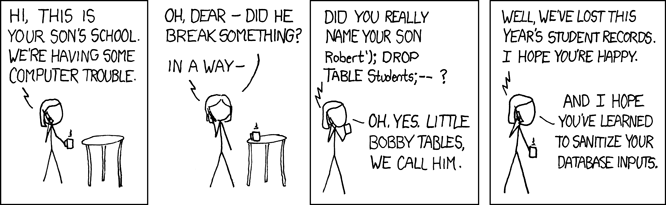
\includegraphics[width=0.95\textwidth]{erros/exploits_of_a_mom.png}
    \fonte{\citeonline{fig_exploits_of_a_mom} / \citeonline{fig_exploits_of_a_mom_explain}.}
    \label{fig:exploits_of_a_mom}
\end{figure}


\section{Erros de modelo de dados}

\begin{itemize}
    \item \erroArmazenarSenhaAberta ;
    
    \item inconsistência na documentação com o método de modelagem utilizado, se a equipe desenvolve a partir de classes utilizando um \ac{orm} que cria as tabelas de forma automática não necessita de um \ac{der}.
    
    \item erro na definição dos modelos apresentados (físico, conceitual, lógico, \ac{der}, \ac{mer}, diagrama de classes);
    
    \item inconsistência entre modelos apresentados (físico, conceitual, lógico, \ac{der}, \ac{mer}, diagrama de classes);

    \item erro na conversão entre modelos;
    
    \item achar que ter um número pequeno de tabelas é mais eficiente que mais tabelas, eficiência tem a ver com modelar corretamente e não com o número de tabelas do banco;
    
    \item dicionário de dados diferente da modelagem apresentada;
    
    \item tipagem de dados incorreta (Ex: um campo para data com tipo VARCHAR);
    
    \item falta de índices adicionais em tabelas do banco de dados, os índices permitem uma busca eficiente sem a leitura completa das tabelas em algumas consultas;
    
    \item falta de teste do modelo definido, muitas vezes não existem campos para armazenamento de informações e também não existem formas de armazenar os dados que se alteram durante o processo e necessitam de histórico;
    
    \item exclusão física de dados que deveriam ser mantidos para histórico;
    
    \item falta de informações para auditoria de processos;
    
    \item erro na escolha de formato de armazenamento de arquivos e imagens (blob ou armazenamento de objetos), cada formato tem vantagens e desvantagens que devem ser considerados de acordo com o contexto da aplicação. Normalmente não faz muito sentido armazenar conteúdos públicos dentro do banco de dados.
    
\end{itemize}

\section{Erros Interface com Usuário}

\begin{itemize}
    \item tradução automática de página via Google tradutor, que acaba gerando falhas de contexto e traduções sem sentido;
    
    \item falta de responsividade em aplicações : web e móvel;
    
    \item não utilizar padrões já existentes para plataforma escolhida;
    
    \item interface complexa para o nível de conhecimento do público alvo da aplicação
    \newline
    \cite{computer_skills}.
    
\end{itemize}

\section{Erros de Validação}

\begin{itemize}
    \item Sistemas de cadastramento que não validam corretamente os dados : falta redigitação de campos importantes como senha;
    
    \item não validar corretamente os campos de acordo com definições existentes (ex e-mail deve seguir \citetitle{rfc5322});
    
    \item falta de validação de e-mail, se o e-mail não for válido o usuário não consegue recuperar a senha (não adianta validar somente o formato, tem que fazer envio com código de validação);
    
    \item falta de sistema seguro para recuperação de senha \cite{forgot_password_cheat_sheet};
    
    \item Limites de senha sem considerar entropia da senha, ex uma senha grande é melhor que uma pequena com diversos tipos de caracteres - \autoref{fig:password_strength};

    \item vulnerabilidade para ataques de injeção - \autoref{fig:exploits_of_a_mom};
    
    \item falta de tratamento no backend, fazendo validações e controle de acesso somente no frontend;
    
\end{itemize}

\begin{figure}
    \centering
    \caption{Boas senhas não devem ser difíceis para o usuário}
	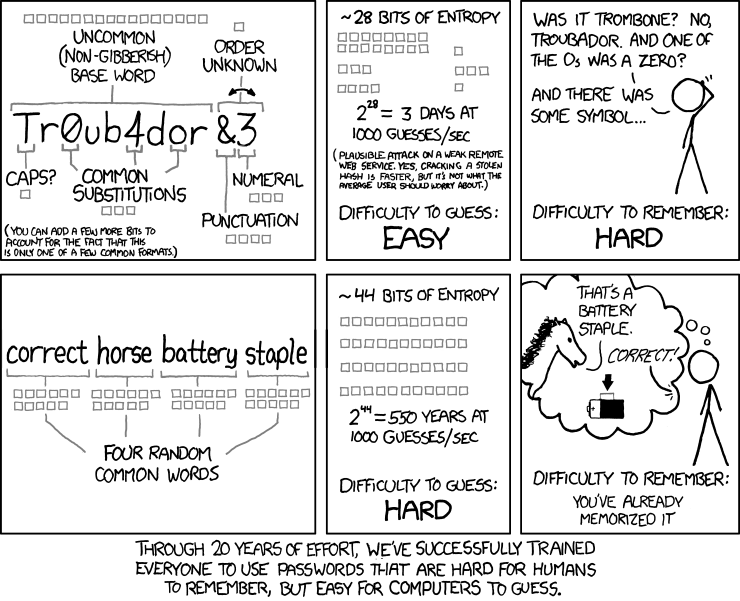
\includegraphics[width=0.95\textwidth]{erros/password_strength.png}
    \fonte{\citeonline{fig_password_strength} / \citeonline{fig_password_strength_explain}.}
    \label{fig:password_strength}
\end{figure}




\section{Erros do processo de teste e apresentação}

\begin{itemize}

    \item testar somente os casos de sucesso sem observar as condições de erro;
    
    \item volume de dados insuficiente para demonstrar o correto funcionamento da aplicação;
    
    \item falta de ordenação nos dados;
    
    \item ordenação sem considerar caracteres de acentuação (ex. Língua deve vir antes de Literatura);
    
% utilizar dados coerentes facilita a apresentação e entendimento da aplicação    
    \item falta de dados consistentes com o contexto da aplicação (escrever teste em um campo pode dificultar posteriormente a analise dos dados).
    
\end{itemize}

\section{Erros de modelagem / análise / projeto}

\begin{itemize}
    \item Casos de uso que não tratam corretamente as ações de usuários, ex recuperação de senha que tem dois passos (solicitar e redefinir senha);
    
    \item definições de casos de uso ou estórias que não detalham claramente o que deve ser feito 
    \newline
    % Instruções exatas como fazer um sanduiche com legendas
    \video{https://www.youtube.com/watch?v=pdhqwbUWf4U}{Como fazer um sanduíche};
    
    \item não analisar corretamente os dados disponíveis para o projeto \cite{boas_perguntas_dados} \cite{guerra-matematica} \cite{ellenberg2015poder} -  \autoref{fig:aviao_wald};
    
    \item desconsiderar o volume de dados e acessos da aplicação ao escolher a arquitetura.
\end{itemize}

\begin{figure}
    \centering
    \caption{Exemplo da análise de \citeonline{wald1980reprint} nos aviões sobreviventes da Segunda Guerra mundial}
	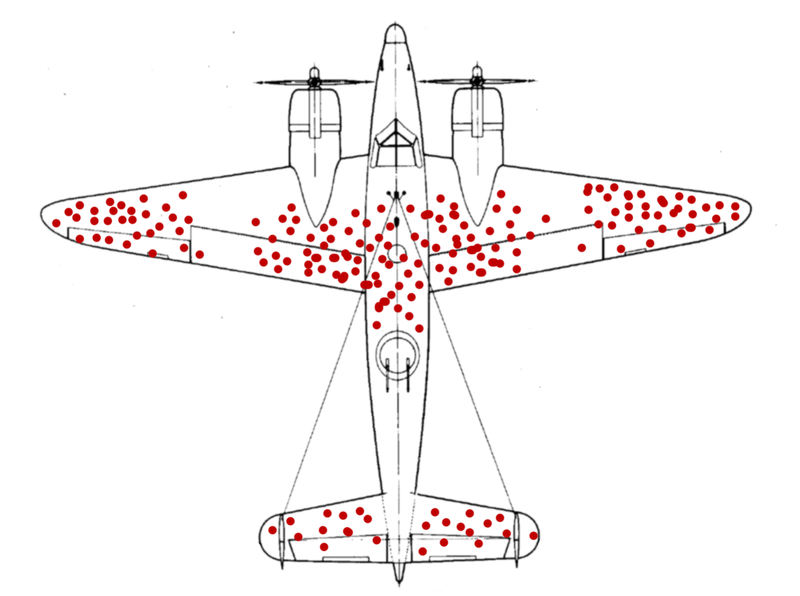
\includegraphics[width=0.8\textwidth]{erros/aviao_wald.png}
    \fonte{\citeonline{fig_aviao_wald}.}
    \label{fig:aviao_wald}
\end{figure}


\section{Erros de planejamento}

\begin{itemize}
    \item Escolher a metodologia X e não utilizar os itens básicos dessa metodologia no desenvolvimento do projeto;
    
    \item escolher \ac{xgh} como metodologia de desenvolvimento \cite{xgh} \cite{xgh-axioms};
    
    \item quem planeja e escolhe a estratégia primeiro tem melhores resultados:
    \begin{itemize}
        \item 
        % Escolha a estratégia correta, corrida sobre tijolos
        \video{https://www.youtube.com/watch?v=4P-i9gCD09s&list=PL69253D27EBEF273E}{Escolha a estratégia correta};
        \item
        % Muito desgate sem planejamento, porquinho buscando cookies sobre geladeira
        \video{https://www.youtube.com/watch?v=LOyX-vgdQGQ&list=PL69253D27EBEF273E}{Muito desgate sem planejamento};
    
        \item % animação : Planejar é Preciso! LEGENDADO
        \video{https://www.youtube.com/watch?v=utLWFdkRm78&list=PL69253D27EBEF273E}{Planejar é Preciso}.    
    \end{itemize}
    
    \item falta de revisão em documentos, aplicação, vídeos;
    
    \item utilizar outras ferramentas e não as obrigatórias das disciplinas, um caso comum é a utilização da ferramenta Postman diretamente (criando a definição manualmente) em vez de utilizar o padrão OpenAPI (swagger) que é obrigatório e que pode ser importado no Postman \cite{postman-openapi};
    
    \item deixar para ultima hora, ex. processos como a criação de documentos no latexdiff, apesar de simples de executar, dependem de preparação de ambiente.
\end{itemize}



\section{Erros de comunicação}

\begin{itemize}
    \item Documentar da melhor maneira para garantir que todos entendam da mesma forma o que deve ser desenvolvido, cuidado com o que escreve:
    \begin{itemize}
        \item \autoref{fig:balanco};
        
        \item \autoref{fig:gabarito-prova};
        
        % Como fazer um sanduiche legendado....
        \item \video{https://www.youtube.com/watch?v=pdhqwbUWf4U&list=PL69253D27EBEF273E}{Como ensinar linguagem de programação para uma criança}.
    \end{itemize}

    \item não acompanhar o e-mail que recebe notificações do \ac{suap}, \gls{moodle};
    
    \item não acompanhar o grupo da disciplina (normalmente no \gls{telegram});
    
    \item falta de comunicação e negociação com os clientes.
\end{itemize}

\todo[inline]{Existem inúmeras versões dessa ilustração \autoref{fig:balanco}, aqui foi utilizada uma publicação como referencia para ilustrar a situação}

\begin{figure}
    \centering
    \caption{A importância da comunicação correta}
	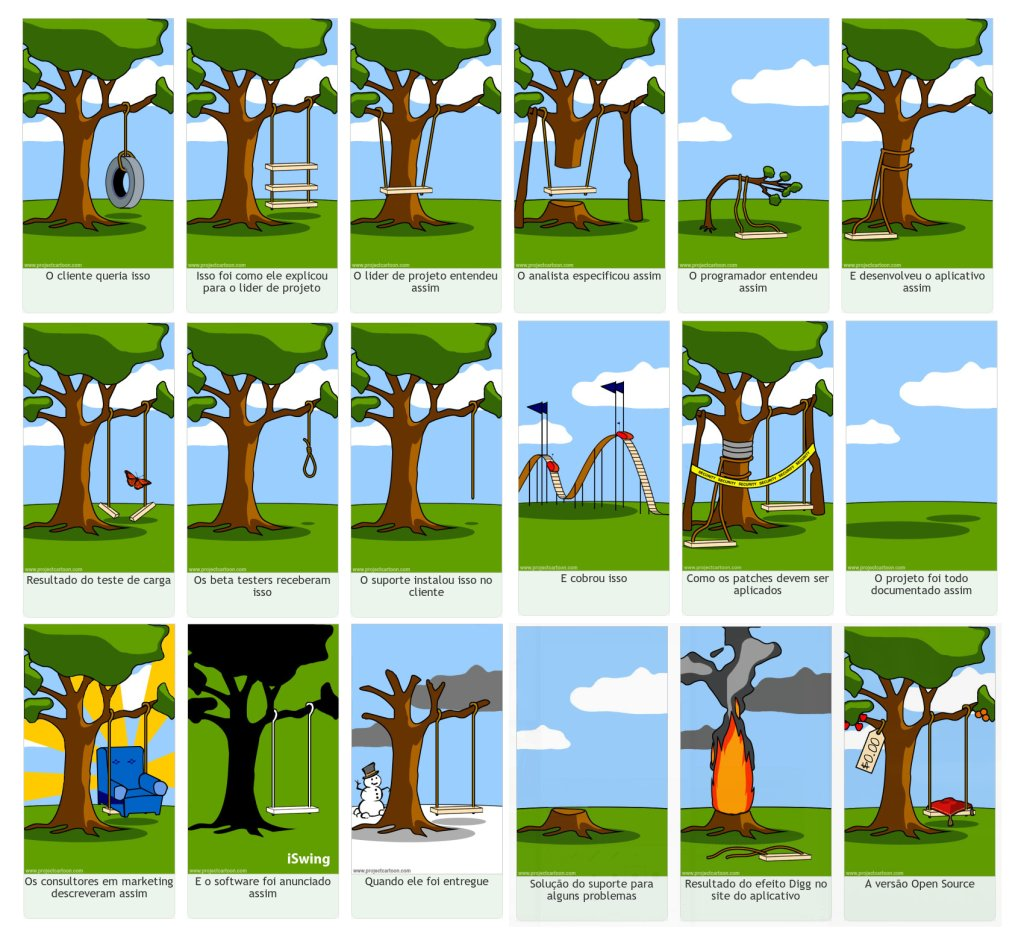
\includegraphics[width=0.95\textwidth]{erros/projeto_balanca_na_arvore.jpg}
    \fonte{\citeonline{engenharia_software_balanca}.}
    \label{fig:balanco}
\end{figure}


\begin{figure}
    \centering
    \caption{A importância da comunicação correta 2}
	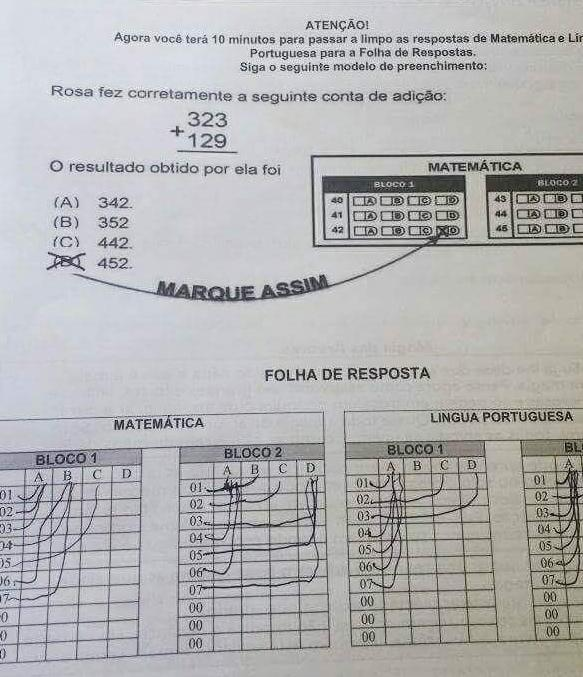
\includegraphics[width=0.95\textwidth]{erros/erro_de_comunicacao_gabarito_prova.jpg}
    \fonte{removida propositalmente.}
    \label{fig:gabarito-prova}
\end{figure}



\section{Erros comportamentais}

Muitos insucessos acontecem devido a comportamentos dos participantes dos projetos, o histórico das disciplinas de projetos demonstraram diversos comportamentos individuais (alguns também acontecem com as equipes) que se evitados permitem melhores resultados:

\begin{itemize}
    \item não escolher os participantes da equipe de acordo com as necessidades do projeto e sim pelas \enquote{amizades} / relações \cite{jackson2019human} \cite{rene_leia_the_human_network} \cite{rene_como_emperrar_a_inovacao};

    \item falta de atenção na leitura dos documentos, regras das disciplinas, mensagens dos professores etc : \autoref{fig:vendo_bolo_cenoura} \cite{atencao_leitura_vendo_bolo_cenoura};
    
    \item medo de errar, para tomar as melhores decisões precisamos de experiencia, e experiencias muitas vezes vem de decisões erradas, mas é importante que essas experiencias aconteçam nos momentos corretos, no inicio e não no final dos projetos \cite{decisions_experience-1} \cite{decisions_experience-2} \autoref{fig:lidar_com_falhas};

    \item não entender o conceito de desenvolvimento de projeto em equipe e responsabilidades: 
    % Diversos videos sobre o trabalho em equipe 
    % Motivacional - Trabalho em equipe - Juntos fazemos mais e melhor!
    \video{https://www.youtube.com/watch?v=twg9SCt76UE&list=PL69253D27EBEF273E}{Trabalho em equipe - Juntos fazemos mais e melhor};
    
    \item não buscar as informações originais que normalmente se encontram em língua inglesa. Muitos documentos da área foram escritos em inglês e possuem traduções com erros técnicos, por isso é importante buscar os documentos originais e não utilizar traduções de terceiros;
    
    \item falta de foco: 
    % A importância de manter o foco!
    % Urso na fila de atendimento....
    \video{https://www.youtube.com/watch?v=6SRTQbBjrFs&list=PL69253D27EBEF273E}{A importância de manter o foco!};
    
    \item focar na tarefa e não no resultado:
    % fazendo trico / cachecol
    \video{https://www.youtube.com/watch?v=J0iv3TqJBV8&list=PL69253D27EBEF273E}{Foco na Tarefa x Foco no Resultado};
    
    \item falta de comprometimento: 
    \autoref{fig:scrum} e 
    \citeonline{meligeni_primeiro_treino};

    \item não acreditar no seu potencial: 
    % Desafio de Gigantes - carregando outro nas costas pelo campo todo...
    \video{https://www.youtube.com/watch?v=7UnyWuu8HK0&list=PL69253D27EBEF273E}{Trecho do filme Desafiando Gigantes - 2006}
    e
    % Rocky Balboa - Motivação Sensacional
    % Outras versões : 
    % https://www.youtube.com/watch?v=JeLYCrE5MrI
    % https://www.youtube.com/watch?v=Rhr6qO7Gmu0
    \video{https://www.youtube.com/watch?v=Qxsyy5H9JTk&list=PL69253D27EBEF273E}{Trecho do filme Rocky Balboa - 2006};
    
    \item medo de sair da zona de conforto:
    % Até a lagosta sente o desconforto do crescimento
    \video{https://www.youtube.com/watch?v=F8VBA89qWpc&list=PL69253D27EBEF273E}{Até a lagosta sente o desconforto do crescimento};
    
    \item falta de motivação, não encarar os desafios, pode ser falta de um \enquote{tubarão} \cite{tubarao_na_vida} \cite{put_a_shark_in_your_tank} \cite{employees_challenge};
    
    \item erro no gerenciamento do tempo e atividades:
    \begin{itemize}
        \item \enquote{macacos no ombro}:
    \waUrl{https://prazercompartilharblog.wordpress.com/2017/09/15/tire-os-macacos-do-meu-ombro/}
    e
    % TIRE O MACACO DO OMBRO
    \video{https://www.youtube.com/watch?v=7alQeDOtiRQ&list=PL69253D27EBEF273E}{TIRE O MACACO DO OMBRO});
    
        \item \video{https://www.youtube.com/watch?v=arj7oStGLkU}{Inside the mind of a master procrastinator} \cite{ted_tim_urban_procastinator}.
    \end{itemize}

    \item deixar para ultima hora o estudo das atividades (latexdiff, statsvn, gource entre outras são ferramentas simples, mas dependem de preparação do ambiente para serem utilizadas);

    \item Não utilizar o conhecimento da equipe para resolver os problemas e fazer as escolhas - \autoref{fig:conhecimento_h2o};
    
    \item Não utilizar os recursos e ferramentas existentes da forma correta - \autoref{fig:uso_recursos_escada_1} e \autoref{fig:uso_recursos_escada_2};

\todo[inline]{Migrar links para referencias e utilizar opções do biblatex}
    \item Não aproveitar os aprendizados de outros alunos que já passaram pelas disciplinas de projetos :
    \begin{itemize}
        \item \waUrlTitle{https://glybif.blogspot.com.br/2016/12/como-ir-bem-em-pds.html}{Como ir bem em PDS? - GLYBIF - 2016};

        \item \waUrlTitle{https://glybif.blogspot.com/2020/04/4-anos-depois-de-fazer-pds.html}{4 anos depois de fazer PDS - GLYBIF - 2020};

        \item \waUrlTitle{https://projetothewalkingpet.blogspot.com/2018/12/dificuldades-e-licoes-aprendidas.html}{Dificuldades e lições aprendidas - The WalkingPet - 2018};

        \item \waUrlTitle{https://projetoa6pgpgrupo101010.blogspot.com/2018/12/o-que-nao-fazer-em-a6pgp-para-que-sofrer.html}{O que NÃO fazer em A6PGP: Para quê sofrer? - Blood 4 Pets - 2018};
        
        \item \waUrlTitle{https://projetoa6pgpgrupo101010.blogspot.com/2018/12/licoes-aprendidas-durante-o-semestre.html}{Lições aprendidas durante o semestre - Blood 4 Pets - 2018};

        \item \waUrlTitle{https://pgppain.blogspot.com/2019/03/19-coisas-que-voce-precisa-saber-sobre.html}{19 coisas que você precisa saber sobre a Prova de Conceito - PGPPain - 2019};

        \item \waUrlTitle{https://pgppain.blogspot.com/2019/03/nos-estamos-atrasados.html}{Nós estamos atrasados - PGPPain - 2019};

        \item \waUrlTitle{https://ginquestapp.wordpress.com/category/dicas-de-sobrevivencia/}{Dicas de Sobrevivência - GinQuest - 2019}.

    \end{itemize}
    
    \item falta de cuidado na comunicação dentro da equipe para garantir o objetivo.
    
\end{itemize}

\begin{figure}
    \centering
    \caption{Erro na interpretação das mensagens ou falta de atenção}
	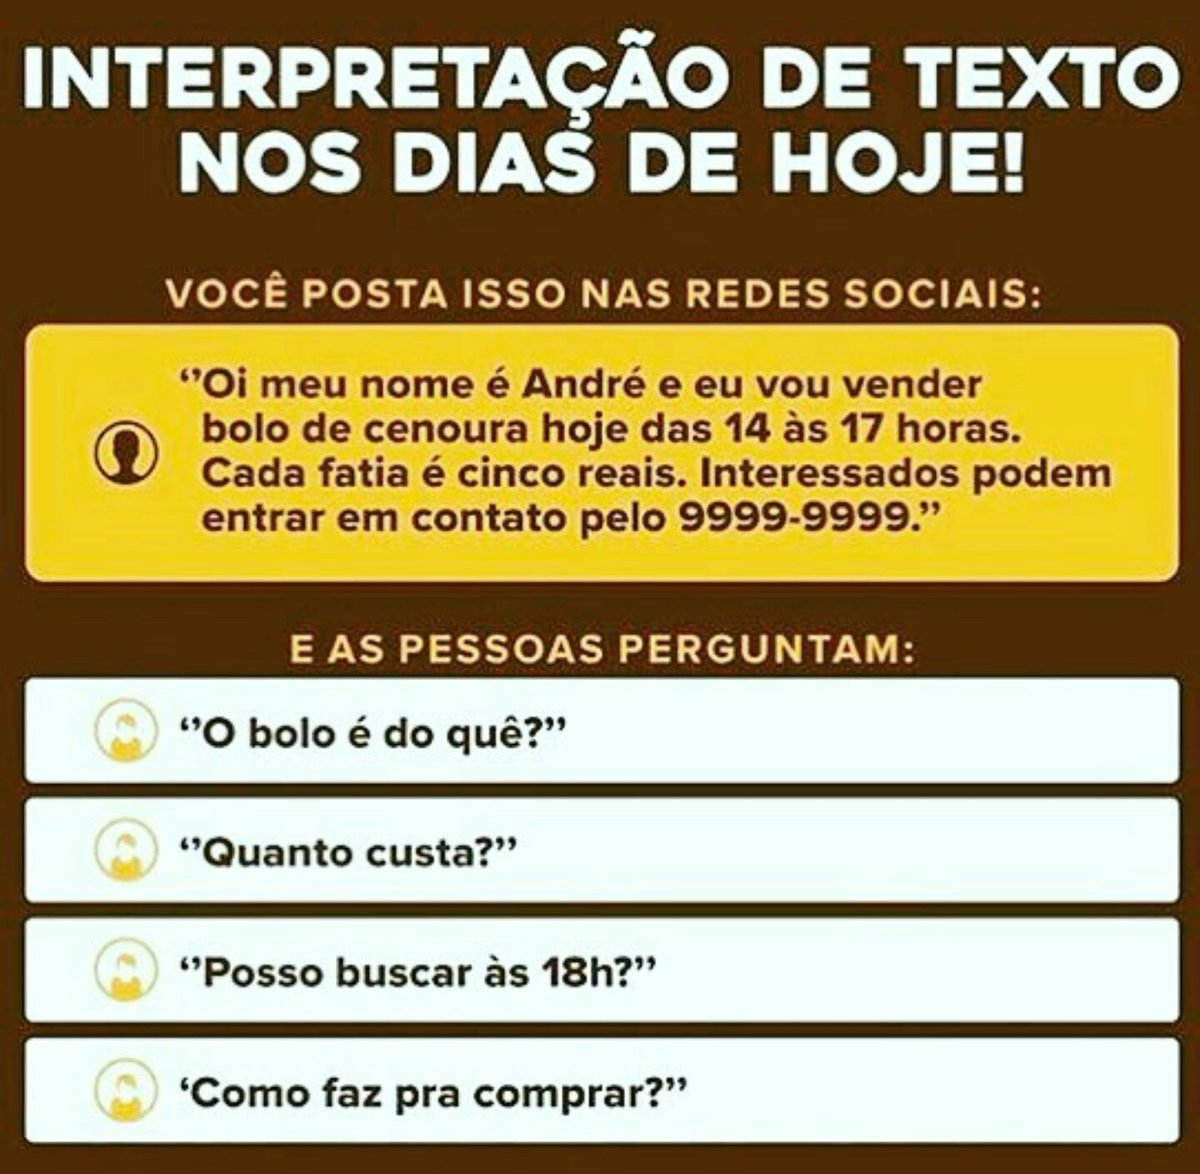
\includegraphics[width=0.95\textwidth]{erros/vendo_bolo_cenoura.jpg}
	\fonte{Autor desconhecido.}
    \label{fig:vendo_bolo_cenoura}
\end{figure}



\begin{figure}
    \centering
    \caption{Comprometimento}
	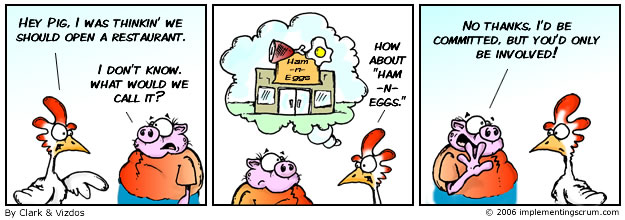
\includegraphics[width=0.95\textwidth]{erros/060911-scrumtoon.jpg}
    \fonte{\citeonline{scrum_cartoon}.}
    \label{fig:scrum}
\end{figure}

\begin{figure}
    \centering
    \caption{Utilizar o conhecimento}
	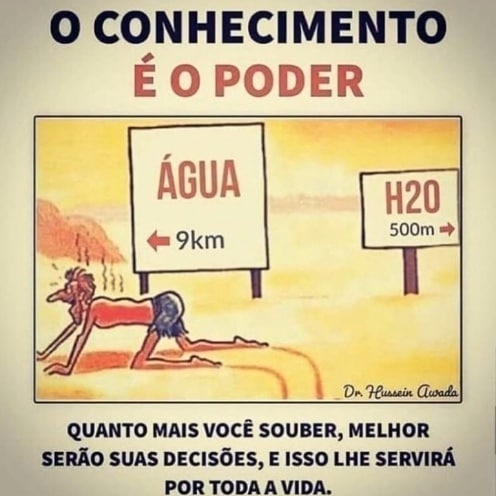
\includegraphics[width=0.7\textwidth]{erros/conhecimento_h2o.jpg}
    \fonte{Hussein Awada, -.}
    \label{fig:conhecimento_h2o}
\end{figure}

\begin{figure}
    \centering
    \caption{Saiba utilizar corretamente seus recursos}
	
\includegraphics[width=0.7\textwidth]{erros/uso_de_recursos_escada_1.jpg}
    \fonte{\citeonline{paulo_maciel_utilizar_recursos}.}
    \label{fig:uso_recursos_escada_1}
\end{figure}

\begin{figure}
    \centering
    \caption{Saiba utilizar corretamente seus recursos - Comparação}
	
\includegraphics[width=0.7\textwidth]{erros/uso_de_recursos_escada_2.jpg}
    \fonte{\citeonline{paulo_maciel_utilizar_recursos_comparado}.}
    \label{fig:uso_recursos_escada_2}
\end{figure}




\begin{figure}
    \centering
    \caption{Aprenda a lidar com suas falhas}
	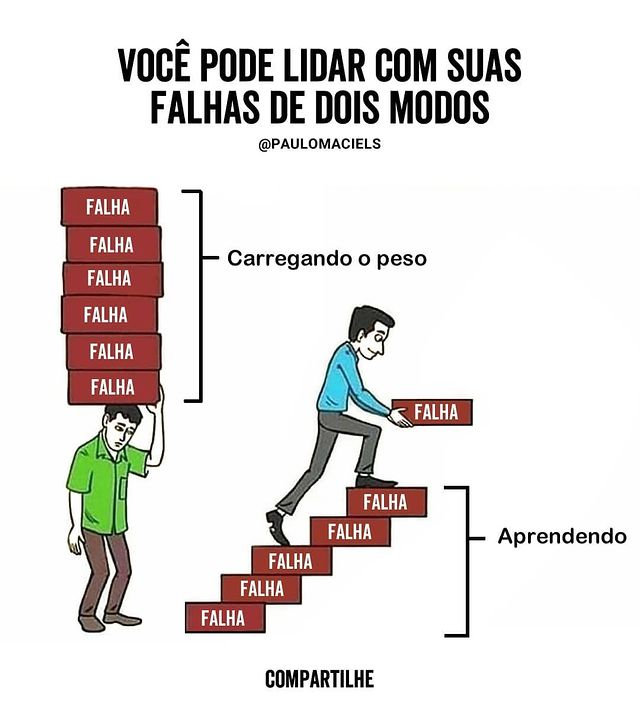
\includegraphics[width=0.7\textwidth]{erros/lidar_com_falhas.jpg}
    \fonte{\citeonline{paulo_maciel_lidar_com_falhas}.}
    \label{fig:lidar_com_falhas}
\end{figure}

